\renewcommand*{\arraystretch}{1.5}
\begin{tabularx}{15cm}{|p{2.1cm}@{\hskip 1ex}|@{\hskip 1ex}X|}
	\hline
	number      & 1                                                          \\ \hline
	title       & Posting summary                                                           \\ \hline
	\multicolumn{2}{|c|}{ 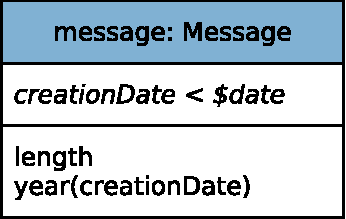
\includegraphics[scale=\patternscale,margin=0cm .2cm]{patterns/q01}} \\ \hline
	description & Given a date, find all Messages created before that date. Group them by
a 3-level grouping:

\begin{enumerate}
\def\labelenumi{\arabic{enumi}.}
\tightlist
\item
  by year of creation
\item
  for each year, group into message types, i.e., Posts or Comments
\item
  for each year-type group, split into four groups based on length of
  their content

  \begin{itemize}
  \tightlist
  \item
    0 \textless{}= length \textless{} 40: \texttt{short}
  \item
    40 \textless{}= length \textless{} 80: \texttt{one\ liner}
  \item
    80 \textless{}= length \textless{} 160: \texttt{tweet}
  \item
    160 \textless{}= length: \texttt{long}
  \end{itemize}
\end{enumerate}
 \\ \hline
	
	group       &
	\multicolumn{1}{>{\raggedright}X|}{
		\varname{year}, 
		\varname{message type}, 
		\varname{length group}
		}\\ \hline
	
	parameters  &
	\multicolumn{1}{>{\raggedright}X|}{
		\variable{date}{Date} 
		}\\ \hline
	result      &
	\multicolumn{1}{>{\raggedright}X|}{
		\variable{message.year}{32bitInteger}\\
		\variable{message type}{String}\\
		\variable{length category}{String}\\
		\variable{message count}{32bitInteger}\\
		\variable{average message length}{32bitInteger}\\
		\variable{sum message length}{32bitInteger}\\
		\variable{per messages}{32bitFloat}
		}\\ \hline
	sort        &
	\multicolumn{1}{>{\raggedright}X|}{
		\sortentry{year}{\desc}\\
		\sortentry{message type}{\asc}\\
		\sortentry{size category}{\asc}
		}\\ \hline
	choke points        &
	\multicolumn{1}{>{\raggedright}X|}{
		\chokepoint{1.2}, 
		\chokepoint{3.2}, 
		\chokepoint{4.1}
		}\\ \hline
\end{tabularx}
\clearpage
